%\begin{figure}[H]
%    \scriptsize
%    \centering
    \setlength{\tabcolsep}{1.5pt}
    \begin{tabular}{cccccc}
        &\footnotesize Bed &\footnotesize Lamp &\footnotesize Lawnmower &\footnotesize Maple Tree &\footnotesize Sunflower\\
        {\rotatebox{90}{\Th{Input}}}&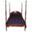
\includegraphics[width=.15\textwidth]{fig/gradient/fig/fig_grad/original/5415.JPEG} &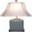
\includegraphics[width=.15\textwidth]{fig/gradient/fig/fig_grad/original/1766.JPEG} &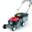
\includegraphics[width=.15\textwidth]{fig/gradient/fig/fig_grad/original/8311.JPEG} &
        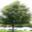
\includegraphics[width=.15\textwidth]{fig/gradient/fig/fig_grad/original/1198.JPEG} & 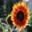
\includegraphics[width=.15\textwidth]{fig/gradient/fig/fig_grad/original/8881.JPEG}\\

        {\rotatebox{90}{\Th{Baseline}}}&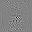
\includegraphics[width=.15\textwidth]{fig/gradient/fig/fig_grad/baseline/5415.JPEG} &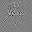
\includegraphics[width=.15\textwidth]{fig/gradient/fig/fig_grad/baseline/1766.JPEG} &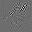
\includegraphics[width=.15\textwidth]{fig/gradient/fig/fig_grad/baseline/8311.JPEG} &
        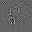
\includegraphics[width=.15\textwidth]{fig/gradient/fig/fig_grad/baseline/1198.JPEG} & 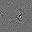
\includegraphics[width=.15\textwidth]{fig/gradient/fig/fig_grad/baseline/8881.JPEG}\\

        {\rotatebox{90}{\Th{Ours}}}&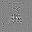
\includegraphics[width=.15\textwidth]{fig/gradient/fig/fig_grad/cosine/5415.JPEG} &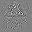
\includegraphics[width=.15\textwidth]{fig/gradient/fig/fig_grad/cosine/1766.JPEG} &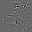
\includegraphics[width=.15\textwidth]{fig/gradient/fig/fig_grad/cosine/8311.JPEG} &
        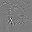
\includegraphics[width=.15\textwidth]{fig/gradient/fig/fig_grad/cosine/1198.JPEG} & 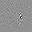
\includegraphics[width=.15\textwidth]{fig/gradient/fig/fig_grad/cosine/8881.JPEG}\\

    \end{tabular}
%    \caption{\textbf{Gradient comparison} of standard \vs our training on CIFAR-100 examples.}
%    \label{fig:grads}
%    \end{figure}